\input{/home/nick/latex-preambles/xelatex.tex}

\newcommand{\imagesPath}{.}

\title{
	\textbf{Δίκτυα Υπολογιστών} \\~\\
	Εργαστηριακή Άσκηση 3 \\ 
	Επικοινωνία στο τοπικό δίκτυο \\
	(πλαίσιο Ethernet και πρωτόκολλο ARP)
}
\author{}
\date{}

\begin{document}
	\maketitle
	
	\begin{tabular}{|l|l|}
		\hline
		\textbf{Ονοματεπώνυμο:} Νικόλαος Παγώνας, el18175 & \textbf{Ομάδα:} 4 (Τρίτη εξ' αποστάσεως) \\
		\hline
		\textbf{Όνομα PC/ΛΣ:} nick-ubuntu/Ubuntu 20.04.3 LTS & \textbf{Ημερομηνία:} Τρίτη 26/10/2021 \\
		\hline
		\textbf{Διεύθυνση IP:} \verb|192.168.1.15| & \textbf{Διεύθυνση MAC:} \verb|3c:2c:30:e1:1c:55|\\
		\hline
	\end{tabular}

	\section*{Άσκηση 1}
		\subsection*{1.1}
			Με την εντολή \verb|ip neigh show| παίρνουμε:
			
			\begin{figure}[H]
				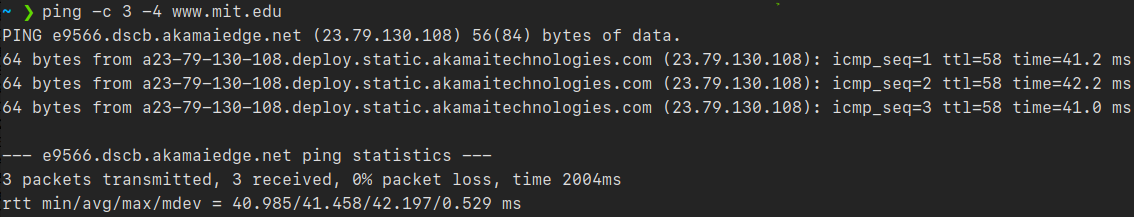
\includegraphics[width=\linewidth]{\imagesPath/1.1.png}
			\end{figure}
			
		\subsection*{1.2}
			Με την εντολή \verb|ip neigh flush all| μπορούμε να διαγράψουμε τα περιεχόμενα του πίνακα ARP, όπως φαίνεται παρακάτω: 
			
			\begin{figure}[H]
				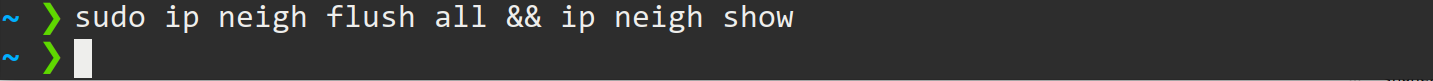
\includegraphics[width=\linewidth]{\imagesPath/1.2.png}
			\end{figure}
		
			Αμέσως μετά το \verb|ip neigh flush all| εκτελέσαμε \verb|ip neigh show| και πήραμε κενή έξοδο, άρα διαγράψαμε τα περιεχόμενα του πίνακα ARP με επιτυχία.
			
		\subsection*{1.3}
			Με τις εντολές \verb+ip route | grep default+ και \verb|resolvectl| βρίσκουμε: 
			
			Την διεύθυνση IPv4 της προκαθορισμένης πύλης:
			
			\begin{figure}[H]
				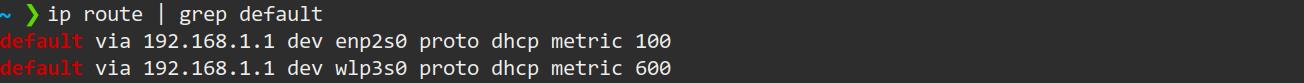
\includegraphics[width=\linewidth]{\imagesPath/1.3.a.png}
			\end{figure}
			
			και την διεύθυνση IPv4 των εξυπηρετητών DNS του υπολογιστή μας:
			
			\begin{figure}[H]
				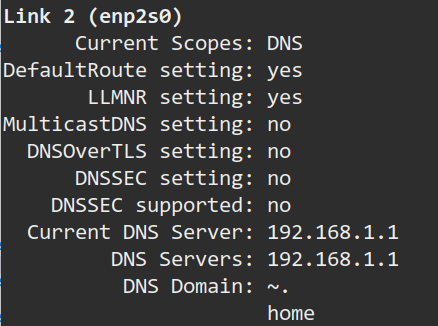
\includegraphics[width=0.4\linewidth]{\imagesPath/1.3.b.png}
			\end{figure}
		
			Βλέπουμε ότι είναι ίδιες (\verb|192.168.1.1|)
			
		\subsection*{1.4}
			
			\begin{figure}[H]
				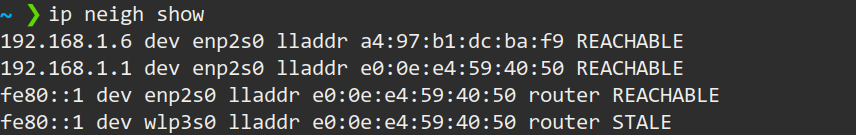
\includegraphics[width=\linewidth]{\imagesPath/1.4.png}
			\end{figure}
			
		\subsection*{1.5}
			Παρατηρούμε ότι η διεύθυνση της προκαθορισμένης πύλης και των εξυπηρετητών DNS (\verb|192.168.1.1|) βρίσκεται στον πίνακα.
			
		\subsection*{1.6}
			Αδειάζουμε τον πίνακα ARP με την εντολή \verb|ip neigh flush all| και στην συνέχεια εκτελούμε \verb|ping 192.168.1.6|.
		
		\subsection*{1.7}
			Αν ξαναεμφανίσουμε τον πίνακα ARP με την εντολή \verb|ip neigh show|, παρατηρούμε ότι η διεύθυνση που κάναμε \verb|ping| ξαναεμφανίστηκε.	
		
		\subsection*{1.8} 
			Έχουν καταχωρηθεί τόσο η διεύθυνση του DNS Server, όσο και του default gateway (αφού είναι ίδιες).
		
		\subsection*{1.9}
			Βλέπουμε ότι η διεύξυνση IPv4 του \verb|edu-dy.cn.ntua.gr| δεν έχει καταχωρηθεί στον πίνακα ARP, αφού βρίσκεται σε διαφορετικό υποδίκτυο.
		
	\section*{Άσκηση 2}
		\subsection*{2.1}
			Καταγράφει τα πεδία \verb|Destination MAC Address|, \verb|Source MAC Address| και \verb|Type|.
		
		\subsection*{2.2}
			Το προοίμιο δεν έχει καταγραφεί, αφού δεν ανήκει στο \textbf{πλαίσιο} Ethernet.
		
		\subsection*{2.3}
			Όπως ξέρουμε, το Wireshark χρησιμοποιεί μία βιβλιοθήκη pcap και άρα έχει πρόσβαση στις δυνατότητες της βιβλιοθήκης αυτής. Τα περισσότερα λειτουργικά συστήματα όμως \textbf{δεν} υποστηρίζουν την καταγραφή του CRC. Ακόμα κι αν την υποστηρίζουν, χρειάζεται ειδικό configuration. Επομένως, είναι λογικό να μην καταγράφεται το CRC. 
		
		\subsection*{2.4}
			Η τιμή του πεδίου Type της επικεφαλίδας Ethernet για πακέτα IPv4 είναι \verb|0x0800|.
		
		\subsection*{2.5}
			Για πακέτα ARP, η τιμή του Type είναι \verb|0x0806|.
		
		\subsection*{2.6}
			Για πακέτα IPv6, η τιμή του Type είναι \verb|0x86dd|.
		
		\subsection*{2.7}
			Η διεύθυνση MAC της πηγής του πλαισίου είναι \verb|3c:2c:30:e1:1c:55|.
		
		\subsection*{2.8}
			H διεύθυνση MAC του προορισμού του πλαισίου είναι \verb|e0:0e:e4:59:40:50|.
		
		\subsection*{2.9}
			Η παραπάνω διεύθυνση MAC δεν είναι αυτή του \verb|edu-dy.cn.ntua.gr|.
		
		\subsection*{2.10}
			Με την εντολή \verb|ip neigh show| βλέπουμε ότι η διεύθυνση MAC ανήκει στο Router του τοπικού μας δικτύου (2η γραμμή). 
			
			\begin{figure}[H]
				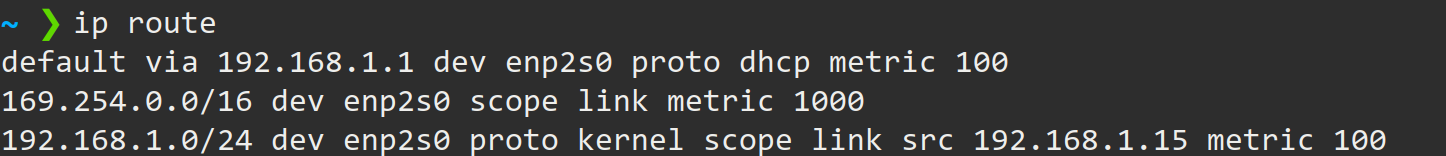
\includegraphics[width=\linewidth]{\imagesPath/2.10.png}
			\end{figure}
		
			Αυτό είναι λογικό, αφού η διεύθυνση του \verb|edu-dy.cn.ntua.gr| είναι εκτός του υποδικτύου στο οποίο βρισκόμαστε, και άρα η επικοινωνία γίνεται μέσω του router.
		
		\subsection*{2.11}
			Το μήκος του πλαισίου είναι 588 bytes.
		
		\subsection*{2.12}
			Προηγούνται συνολικά 66 bytes.
		
		\subsection*{2.13}
			Η διεύθυνση MAC του αποστολέα είναι η \verb|e0:0e:e4:59:40:50|.
		
		\subsection*{2.14}
			Η παραπάνω διεύθυνση δεν είναι η διεύθυνση MAC του \verb|edu-dy.cn.ntua.gr|.
		
		\subsection*{2.15}
			Η διεύθυνση αυτή είναι και πάλι η διεύθυνση του router του τοπικού μας δικτύου.
		
		\subsection*{2.16}
			Η διεύθυνση MAC του παραλήπτη είναι \verb|3c:2c:30:e1:1c:55|.
		
		\subsection*{2.17}
			Η διεύθυνση αυτή ανήκει στον υπολογιστή μας.
		
		\subsection*{2.18}
			Το μήκος του πλαισίου είναι 549 bytes.
		
		\subsection*{2.19}
			Προηγούνται πάλι 66 bytes.

	\section*{Άσκηση 3}
	
		\subsection*{3.1}
			Παρατηρούμε ότι οι διευθύνσεις MAC πηγής των πλαισίων Ethernet είναι individual και globally unique.
			
		
		\subsection*{3.2} 
			Παρατηρούμε ότι οι διευθύνσεις MAC προορισμού των πλαισίων Ethernet είναι group, ενώ όσον αφορά το LG έχουμε και locally administered και globally unique
		
		\subsection*{3.3}
			Το πρώτο bit της διεύθυνσης MAC (IG bit) εμφανίζεται στην 8η θέση του πρώτου byte (δηλαδή στο LSB) \verb|(____ ___x)|, ενώ το δεύτερο bit (LG bit) εμφανίζεται στην 7η θέση \verb|(____ __x_)|. 
		
		\subsection*{3.4}
			Η διεύθυνση MAC για τα πλαίσια εκπομπής (broadcast) είναι \verb|ff:ff:ff:ff:ff:ff|.
		
		\subsection*{3.5}
			Παραμένουν πλαίσια IEEE 802.3 (περιέχουν επικεφαλίδα \textbf{L}ogical \textbf{L}ink \textbf{C}ontrol, εξού και το όνομα του φίλτρου).
		
		\subsection*{3.6}
			Στα πλαίσια IEEE 802.3, το πεδίο μετά τις διευθύνσεις MAC (\verb|Length|) δηλώνει πόσα byte περιέχονται στο πεδίο δεδομένων.
		
		\subsection*{3.7}
			Τα πλαίσια ΙΕΕΕ 802.3 ξεχωρίζουν από τα Ethernet II ως εξής:
				\begin{itemize}
					\item Στο Wireshark το πλαίσιο αναγράφεται ως IEEE 802.3 αντί για Ethernet II 
					\item Στη θέση του πεδίου \verb|Type| (Ethernet II) βρίσκεται το πεδίο \verb|Length| (IEEE 802.3), το οποίο ξεχωρίζει διότι οι τιμές του πεδίου \verb|Type| είναι μεγαλύτερες από 1536 (0x0600)
					\item Μετά το \textit{Μήκος}, τα πλαίσια IEEE 802.3 περιέχουν μία επικεφαλίδα LLC, όπως αναφέρεται και στην θεωρία.
				\end{itemize}
		
		\subsection*{3.8}
			Η επικεφαλίδα LLC έχει μέγεθος 3 byte και περιλαμβάνει τα πεδία \verb|DSAP|, \verb|SSAP| και \verb|Control Field|.
		
		\subsection*{3.9}
			Του Spanning Tree Protocol, 36 bytes
		
		\subsection*{3.10}
			Το παραγέμισμα έχει μήκος 7 bytes και υπάρχει σε περιπτώσεις που τα πλαίσια είναι πολύ μικρά, ώστε να ικανοποιείται το πρότυπο IEEE 802.3, το οποίο υπαγορεύει ελάχιστο μήκος πλαισίου 64 bytes.

	\section*{Άσκηση 4}
		\textbf{Σημείωση}: Επειδή το μηχάνημα που χρησιμοποιήσαμε στην άσκηση 1 δεν ήταν διαθέσιμο κατά την διάρκεια εκτέλεσης της Άσκησης 4, χρησιμοποιήσαμε μία άλλη συσκευή με IPv4 address 192.168.1.7.
		
		\subsection*{4.1}
			Η εφαρμογή αυτού του φίλτρου έχει αποτέλεσμα να δείχνει μόνο τα πακέτα που έστειλε/έλαβε η κάρτα δικτύου μας.
			
		
		\subsection*{4.2}
			Η εφαρμογή του δεύτερου φίλτρου περιορίζει περαιτέρω το αποτέλεσμα του πρώτου, με τον επιπλέον συνθήκη ότι τα πακέτα πρέπει να ενθυλακώνουν το πρωτόκολλο ARP.
		
		\subsection*{4.3}
			Ανταλλάχθηκαν 2 πακέτα.
		
		\subsection*{4.4}
			Το πεδίο που τα διαφοροποιεί είναι το Type (έχει τιμή \verb|0x0806|)
		
		\subsection*{4.5}
			\begin{itemize}
				\item Hardware Type: 2 bytes
				\item Protocol Type: 2 bytes 
				\item Hardware Size: 1 byte
				\item Protocol Size: 1 byte
				\item Opcode: 2 bytes
				\item Sender MAC Address: 6 bytes
				\item Sender IP Address: 4 bytes
				\item Target MAC Address: 6 bytes
				\item Target IP Address: 4 bytes
				\item Padding: 18 bytes				
			\end{itemize}
		
		\subsection*{4.6}
			Η τιμή του πεδίου \verb|Hardware Type| είναι 1 και υποδεικνύει κάρτα δικτύου Ethernet.
			
		
		\subsection*{4.7}
			Η τιμή του πεδίου \verb|Protocol Type| είναι \verb|0x0800| και υποδεικνύει πρωτόκολλο IPv4 
			
		
		\subsection*{4.8}
			Υπάρχει 1-1 αντιστοιχία, για παράδειγμα αν η τιμή του πεδίου \verb|Protocol Type| είναι \verb|0x0800|, τότε και η αντίστοιχη τιμή του πεδίου \verb|EtherType| θα είναι \verb|0x0800|.
			
		
		\subsection*{4.9}
			Η τιμή του πεδίου \verb|Protocol Size| έχει την τιμή 4, διότι έχουμε να κάνουμε με IPv4 πακέτα, και οι IPv4 διευθύνσεις έχουν μήκος 4 bytes. 
		
		\subsection*{4.10}
			Αντίστοιχα, η τιμή του πεδίου \verb|Hardware Size| είναι 6, διότι οι MAC διευθύνσεις έχουν μήκος 6 bytes.
		
		\subsection*{4.11}
			Η διεύθυνση MAC αποστολέα του πλαισίου Ethernet που μεταφέρει το ARP Request ανήκει στον υπολογιστή μας.	
		
		\subsection*{4.12}
			Η διεύθυνση MAC του παραλήπτη είναι \verb|ff:ff:ff:ff:ff:ff|.
		
		\subsection*{4.13}
			Το συνολικό μέγεθος του πακέτου ARP Request είναι 28 bytes, ενώ του πλαισίου Ethernet που το μεταφέρει είναι 42 bytes.
		
		\subsection*{4.14}
			Προηγούνται 20 bytes.
		
		\subsection*{4.15}
			Η τιμή του πεδίου opcode στο ARP Request είναι 1.
		
		\subsection*{4.16}
			Περιέχεται στο Sender MAC Address.
		
		\subsection*{4.17}
			Περιέχεται στο Sender IP Address.
		
		\subsection*{4.18}
			Περιέχεται στο Target IP Address.
		
		\subsection*{4.19}
			Υπάρχει το Target MAC Address, με τιμή \verb|00:00:00:00:00:00|.
		
		\subsection*{4.20}
			Η διεύθυνση MAC του αποστολέα ανήκει στο μηχάνημα που κάναμε ping, ενώ του παραλήπτη ανήκει στο δικό μας μηχάνημα.
		
		\subsection*{4.21}
			Η τιμή του πεδίου opcode στο ARP Reply είναι 2.
		
		\subsection*{4.22}
			Περιέχεται στο Sender IP Address.
		
		\subsection*{4.23}
			Περιέχεται στο Sender MAC Address.
		
		\subsection*{4.24}
			Περιέχεται στο Target IP Address.
		
		\subsection*{4.25}
			Περιέχεται στο Sender MAC Address.
		
		\subsection*{4.26}
			Το συνολικό μέγεθος σε byte του πακέτου ARP Reply είναι 28 bytes, ενώ του πλαισίου Ethernet που το μεταφέρει 60 bytes.
		
		\subsection*{4.27}
			Παρατηρούμε ότι δεν είναι ίδια.
		
		\subsection*{4.28}
			Στην περίπτωση που στέλνουμε το ARP Request, το padding γίνεται ακριβώς πριν μεταδοθεί το πακέτο, επομένως το Wireshark δεν μπορεί να το καταγράψει. Αντιθέτως, όταν λαμβάνουμε το ARP Reply, το padding έχει ήδη γίνει από την πλευρά του αποστολέα, οπότε το Wireshark το καταγράφει. Γι' αυτό έχουμε διαφορές στο μέγεθος πακέτου μεταξύ των δύο περιπτώσεων.
		
		\subsection*{4.29}
			Το πεδίο opcode (1 για request, 2 για reply)
		
		\subsection*{4.30}
			Στο request έχουμε multicast/broadcast και locally administered address, ενώ στο reply έχουμε globally unique address και unicast (πάντα μιλάμε για το Destination).
			
		\subsection*{4.31}
			Τότε όλοι οι χρήστες θα έστελναν τα πακέτα τους στον κακόβουλο χρήστη, νομίζοντας ότι τα στέλνουν εκεί που αρχικά ήθελαν, θέτοντας σε κίνδυνο τα δεδομένα τους.
\end{document}